\documentclass[a4paper,12pt]{article}
\usepackage[a4paper,top=1.3cm,bottom=2cm,left=1.5cm,right=1.5cm,marginparwidth=0.75cm]{geometry}
\usepackage{cmap}
\usepackage{mathtext}
\usepackage[T2A]{fontenc}
\usepackage[utf8]{inputenc}
\usepackage[english,russian]{babel}
\usepackage{siunitx}

\usepackage{graphicx}

\usepackage{wrapfig}
\usepackage{tabularx}
\usepackage{multirow}

\usepackage{hyperref}
\usepackage[rgb]{xcolor}
\hypersetup{
colorlinks=true,urlcolor=blue
}
\usepackage{amsmath,amsfonts,amssymb,amsthm,mathtools}
\usepackage{icomma}
\mathtoolsset{showonlyrefs=false}
\usepackage{euscript}
\usepackage{mathrsfs}
\DeclareMathOperator{\sgn}{\mathop{sgn}}
\newcommand*{\hm}[1]{#1\nobreak\discretionary{}
{\hbox{$\mathsurround=0pt #1$}}{}}

%%% Заголовок
\author{Макаров Лев Евгеньевич}
\title{Лабораторная работа №2.1.1

Изучение экспериментальных погрешностей на примере физического маятника
}
\date{\today}

\begin{document}

\begin{titlepage}
	\begin{center}
		{\large МОСКОВСКИЙ ФИЗИКО-ТЕХНИЧЕСКИЙ ИНСТИТУТ (НАЦИОНАЛЬНЫЙ ИССЛЕДОВАТЕЛЬСКИЙ УНИВЕРСИТЕТ)}
	\end{center}
	\begin{center}
		{\large Физтех-школа фотоники, электроники и молекулярной физики}
	\end{center}
	
	
	\vspace{4.5cm}
	{\huge
		\begin{center}
			{\bf Отчёт о выполнении лабораторной работы 2.1.1}\\
			Измерение удельной теплоёмкости воздуха при постоянном давлении
		\end{center}
	}
	\vspace{2cm}
	\begin{flushright}
		{\LARGE Автор:\\ Макаров Лев Евгеньевич \\
			\vspace{0.2cm}
			Б04-306}
	\end{flushright}
	\vspace{8cm}
	\begin{center}
		Долгопрудный 2024
	\end{center}
\end{titlepage}

\section{Введение}

\textbf{Цель работы:} 
\begin{enumerate}
	\item измерить повышение температуры воздуха в зависимости от мощности подводимого тепла и расхода при стационарном течении через трубу;
    \item исключив тепловые потери, по результатам измерений определить теплоёмкость воздуха при постоянном давлении
\end{enumerate}

\textbf{В работе используются:} 
\begin{itemize}
    \item теплоизолированная стеклянная трубка
    \item электронагреватель
    \item источник питания постоянного тока
    \item амперметр, вольтметр (цифровые мультиметры) 
    \item термопара, подключенная к микровольтметру
    \item компрессор
    \item газовый счётчик
    \item секундомер
\end{itemize}
\medskip

\section{Теоретические сведения}

\subsection{Теория}

Измерение теплоёмкости тел обычно производится в калориметрах. При этом регистрируется изменение его температуры $ d T $ в зависимости от количества тепла $ \delta Q $, полученного телом от некоторого нагревательного элемента внутри калориметра. Теплоёмкость тела в некотором процессе определяется как их отношение:

\begin{equation}
    C = \frac{\delta Q}{ d T }
\end{equation}

Надёжность измерения определяется, в основном, качеством калориметра. Необходимо, чтобы количество тепла, затрачиваемое на нагревание исследуемого тела, существенно превосходило тепло, расходуемое на нагревание самого калориметра, а также на потери тепла из установки. При измерении теплоёмкости газов эти требования выполнить довольно трудно — масса газа в калориметре и количество тепла, идущее на его нагревание малы. Для увеличения количества нагреваемого газа при неизменных размерах установки в нашей работе исследуемый газ (воздух) продувается через калориметр, внутри которого установлен нагреватель. При этом измеряются мощность нагревателя, масса воздуха, протекающего в единицу времени (расход), и приращение его температуры.

\begin{wrapfigure}{r}{0.5\linewidth}
    \centering
    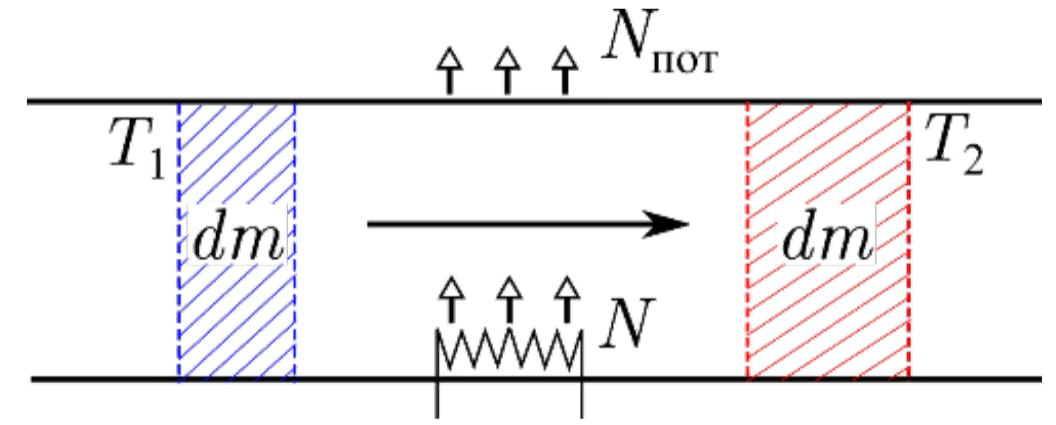
\includegraphics[height=3cm]{nagrev.png}
    \caption{\textit{Нагрев газа при течении по трубе}}
    \label{fig:myfig1}
\end{wrapfigure}

Рассмотрим газ, протекающий стационарно слева направо через трубу постоянного сечения, в которой установлен нагревательный элемент (см. рис. 1). Пусть за некоторое время $dt$ через калориметр прошла малая порция газа массой $dm=qdt$, где q [кг/с] — массовый расход газа в трубе. Если мощность нагрева равна N, мощность тепловых потерь на обмен с окружающей средой $N_\text{пот}$, то порция получила тепло $\delta Q = (N-N_\text{пот})dt$. С другой стороны, по определению теплоёмкости (1): $\delta Q = c dm \Delta T$, где $\Delta T$ — приращение температуры газа, и c — удельная (на единицу массы) теплоёмкость газа в рассматриваемом процессе. При малых расходах газа и достаточно большом диаметре трубы перепад давления на её концах мал, поэтому можно принять, что $P_1 \approx P_2 = P_0$, где $P_0$ — атмосферное давление. Следовательно, в условиях опыта измеряется удельная теплоёмкость при постоянном давлении $c_p$. Таким образом, получаем

\begin{equation}
    c_p = \frac{N-N_\text{пот}}{q \Delta T}
\end{equation}

Более подробное рассмотрение позволяет установить, что формула (2) справедлива даже в том случае, если перепад давлений на концах трубы не мал, при условии, что газ можно считать идеальным, а его кинетической энергией можно пренебречь. Кроме того, для практического использования (2) должны быть малы потери тепла и тепловыделение из-за трения (по сравнению с мощностью нагревателя).

\subsection{Методика измерений}

В настоящем эксперименте предлагается провести измерение зависимости $\Delta T (N)$ разности температур $\Delta T$ концов термопары от мощности нагрева $N = UI$ при нескольких фиксированных значениях расхода q воздуха. По результатам измерений проверить справедливость зависимости (10) и определить удельную теплоёмкость воздуха при постоянном давлении $c_p$, а также оценить величину тепловых потерь. Важнейшим условием корректности проведение опыта является установление стационарного состояния. Снятие показаний рекомендуется производить когда показания вольтметра, подключенного к термопаре, не меняются в течение 1-2 минут. Кроме того, необходимо учитывать, что охлаждение системы занимает существенно большее время, нежели нагрев, поэтому при измерениях мощность нагрева нужно увеличивать постепенно. Охлаждение установки для повторного снятия зависимости производится при максимальном расходе воздуха и выключенном нагревателе.

\section{Оборудование и экспериментальные погрешности}

\textbf{Амперметр:} $\sigma_\text{A} = 0,03$ мА \\
\textbf{Генератор:} $\sigma_\text{V} = 0,003$ В \\
\textbf{Вольтметр:} $\sigma_\text{V} = 0,003$ мВ \\
\textbf{Секундомер:} $\sigma_\text{s} = 0,6$ с \\
\textbf{Газовый счётчик:} $\sigma_\text{s} = 0,02$ л \\
\textbf{Термометр:} $\sigma_\text{t} = 0,3$ дцПа \\
\textbf{Манометр:} $\sigma_\text{p} = 0,3$ $C^\circ$ \\

Схема установки изображена на рис. \ref{fig:myfig1}. Воздух, нагнетаемый компрессором, прокачивается через калориметр. Калориметр представляет собой стеклянную цилиндрическую трубку с двойными стенками, запаянными с торцов. На внутреннюю поверхность стенок трубки нанесено серебряное покрытие. Воздух из пространства между стенками калориметра откачан до высокого вакуума ($10^{-5} $ торр).

\begin{figure}[h]
    \begin{center}$
        \begin{array}{cc}
            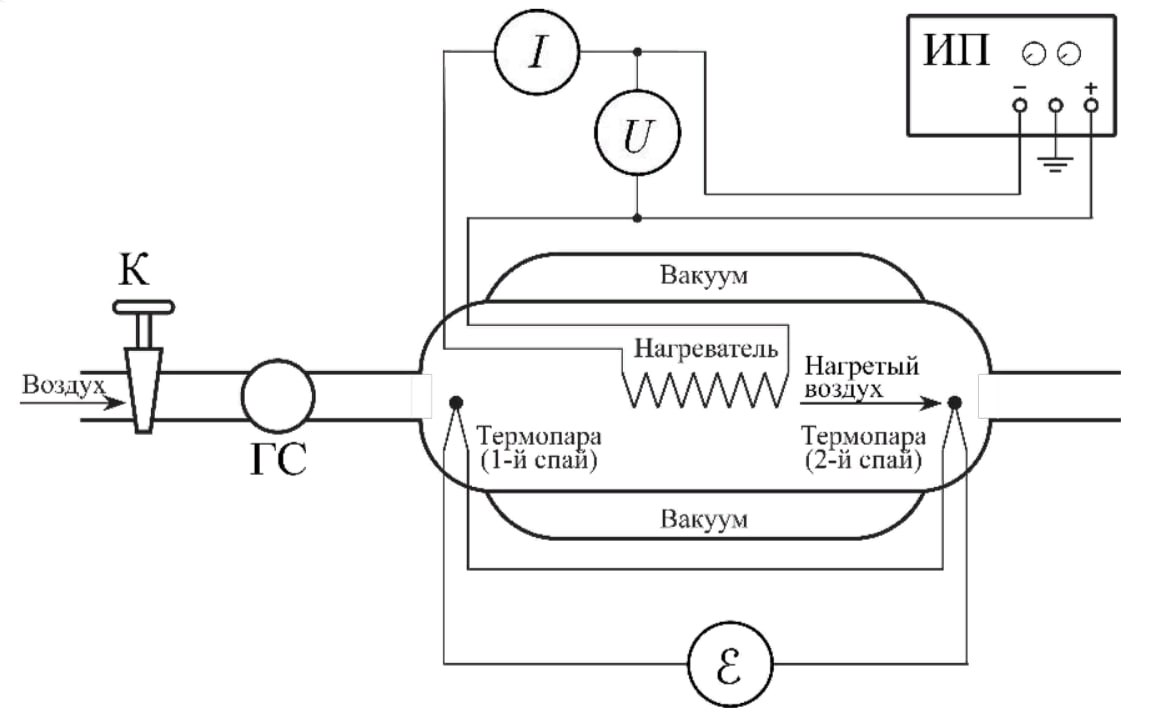
\includegraphics[width=0.8\textwidth]{ustan.png}\\
        \end{array}$
    \end{center}
    \caption{\text{Схема экспериментальной установки}}
\end{figure}

Нагреватель расположен внутри калориметра непосредственно в воздушном потоке. Нагрев производится от регулируемого источника постоянного тока (ИП). Напряжение $U$ на нагревателе и ток $I$ через него регистрируются цифровыми мультиметрами. Таким образом, мощность нагрева равна

\begin{equation}
    N = UI
\end{equation}

Для измерения разности температур $\Delta T$ служит медно-константановая термопара. Один спай термопары расположен в струе воздуха, входящего в калориметр, и находится при комнатной температуре, а второй — в струе выходящего нагретого воздуха. Константановая проволока термопары расположена внутри калориметра, а медные проводники подключены к цифровому вольтметру. Возникающая в термопаре ЭДС $\varepsilon$ пропорциональна разности температур $\Delta T$ спаев:

\begin{equation}
    \varepsilon = \beta \Delta T    
\end{equation}

где $\beta = 40,7 \frac{мкВ}{C^{\circ}}$— чувствительность медно-константановой термопары в рабочем диапазоне температур (20–30 ℃). ЭДС регистрируется с помощью микровольтметра. Объём воздуха, прошедшего через калориметр, измеряется газовым счётчиком ГС. Для регулировки расхода служит кран К. Время $\Delta t$ прохождения некоторого объема $\Delta V$ воздуха измеряется секундомером. Объёмный расход равен $\frac{\Delta V}{\Delta t}$, массовый расход может быть найден как

\begin{equation}
    q = \rho_0 \frac{\Delta V}{\Delta t}
\end{equation}

где $\rho_0$ — плотность воздуха при комнатной температуре. Можно предположить, что при небольшом нагреве мощность потерь тепла $N_\text{пот}$ прямо пропорциональна разности температур:

\begin{equation}\label{loss}
    N = \alpha \Delta T
\end{equation}

где $\alpha$ — некоторая константа. При этом условии основное соотношение (2) принимает вид

\begin{equation}\label{find-a}
    N = (c_p q + \alpha) \Delta T
\end{equation}

Следовательно, при фиксированном расходе воздуха (q = const) подводимая мощность и разность температур связаны прямой пропорциональностью.

\section{Результаты измерений и обработка данных}

\subsection{Подготовка газового счётчика}

Газовый счётчик был заранее подготовлен к работе лаборантом.

\subsection{Охлаждение калориметра}

Включим комрессор, открыв кран К. Установим максимально возможный расход воздуха (полный оборот стрелка совершает за 30 секунд). Так как стрелка вращается равномерно, значит газовый счётчик работает корректно.

\subsection{Подготовка приборов}

Включим вольтметр, будем продувать калориметр пока значение вольтметра не станет равным нулю.

\subsection{Определение плотности воздуха}
    
Запишем показания температуры и давления воздуха. 

\begin{equation}
    T = (23,6 \pm 0,3) \ C^\circ \ \ \ P = (959,3 \pm 0,3) \text{ дцПа} 
\end{equation}

Плотность воздуха в комнате вычислим по формуле ($\mu = 29.0$ г/моль):

\begin{equation}
    \rho_0 = \frac{\mu P}{RT} = \frac{0,029 \cdot 95930}{8,31 \cdot 297,4} = 1,131 \ \text{кг}/\text{м}^3
\end{equation}

Погрешность измерения можно вычислить по формуле:

\begin{multline*}
    \sigma_{\rho_0} = \sqrt{
    \left ( \frac{\partial \rho_0}{\partial P} \right )^2 \sigma_{P} ^ 2 +
    \left ( \frac{\partial \rho_0}{\partial T} \right )^2 \sigma_{T} ^ 2
    } = \sqrt{
    \left ( \frac{\mu}{RT} \right )^2 \sigma_{P} ^ 2 + 
    \left ( \frac{\mu P}{RT^2} \right )^2 \sigma_{T} ^ 2
    } = \frac{\mu}{RT} \sqrt{ \sigma_{P} ^ 2 + \left( \frac{P}{T} \right)^2 \sigma_{T} ^ 2} = 
\end{multline*}

\begin{equation}
    = \frac{0,029}{8,31 \cdot 297,4} \sqrt{ 30 ^ 2 + \left( \frac{30}{297,36} \right)^2 0,3 ^ 2} = 0,001 \ \text{кг}/\text{м}^3
\end{equation}

Таким образом плотность воздуха $\rho_0 = (1,131 \pm 0,001) \ \text{кг}/\text{м}^3$.

\subsection{Определение расхода}
\label{find-q}

Для измерения точного расхода будем с помощью секундомера замерять за сколько секунд прошёл определённый объём воздуха. Замерения будем делать каждый оборот стрелки (каждые 5 л), результаты запишем в таблицу \ref{q1}. Сразу посчитаем массовый расход, разделив объёмный на плотность. Таким образом расход определяется по формуле:

\begin{equation}
    q = \frac{V}{T \rho_0}
\end{equation}

\begin{table}[!ht]
    \centering
    \begin{tabular}{|l|l|l|l|l|l|l|}
    \hline
        $N$ & $V$, л & $T$, с & $q$, л/с & $q$, г/с & $\sigma_q$, г/с & $\varepsilon_q$, \% \\ \hline
        1 & 5,00 & 33,0 & 0,151 & 0,1711 & 0,0025 & 1,46 \\ \hline
        2 & 10,00 & 65,9 & 0,152 & 0,1716 & 0,0013 & 0,73 \\ \hline
        3 & 15,00 & 98,8 & 0,152 & 0,1716 & 0,0008 & 0,49 \\ \hline
        4 & 20,00 & 131,6 & 0,152 & 0,1719 & 0,0006 & 0,37 \\ \hline
        5 & 25,00 & 164,4 & 0,152 & 0,1719 & 0,0005 & 0,30 \\ \hline
        6 & 30,00 & 197,5 & 0,152 & 0,1718 & 0,0004 & 0,26 \\ \hline
        7 & 35,00 & 230,3 & 0,152 & 0,1718 & 0,0004 & 0,22 \\ \hline
    \end{tabular}\caption{\textit{Измерение расхода газа $q_1$}}\label{q1}
\end{table}

Тогда приборную погрешнсоть можно вычислить по формуле:

\begin{multline*}
    \sigma_q^\text{приб} = \sqrt{
    \left ( \frac{\partial q}{\partial V} \right )^2 \sigma_{V} ^ 2 +
    \left ( \frac{\partial q}{\partial T} \right )^2 \sigma_{T} ^ 2 +
    \left ( \frac{\partial q}{\partial \rho_0} \right )^2 \sigma_{\rho_0} ^ 2
    } = \sqrt{
    \left ( \frac{1}{T \rho_0} \right )^2 \sigma_{V} ^ 2 +
    \left ( \frac{V}{T^2 \rho_0} \right )^2 \sigma_{T} ^ 2 +
    \left ( \frac{V}{T \rho_0^2} \right )^2 \sigma_{\rho_0} ^ 2
    }
\end{multline*}

\begin{equation}\label{sigma-q}
    \sigma_q^\text{приб} = \frac{1}{T \rho_0} \sqrt{
    \sigma_{V} ^ 2 +
    \left ( \frac{V}{T} \right )^2 \sigma_{T} ^ 2 +
    \left ( \frac{V}{\rho_0} \right )^2 \sigma_{\rho_0} ^ 2
    }
\end{equation}

Для каждого измерения в таблице вычислим погрешность, запишем её в таблицу \ref{q1}. Сразу посчитаем относительную погрешность и запишем её в таблицу \ref{q1}.

Среднее значение расхода $\overline{q_1} = 0,172 \ \text{г}/\text{с}$. Тогда случайную погрешность можно вычислить по формуле:

\begin{equation}
    \sigma_q^\text{случ} = \sqrt{\frac{1}{N  (N-1)}\sum(q_{1i}-\overline{q_1})^2} \approx 0,0001 \ \text{г}/\text{с}
\end{equation}

Видно, что случайная погрешность измерения сильно меньше приборной, а значит ей можно пренебречь.

Таким образом расход газа равен

\begin{equation}
    q_1 = (0,172 \pm 0,001) \ \text{г}/\text{с}
\end{equation}

\subsection{Оценка значения тока}
\label{N-I-0}

Смесь двухатомных идеальных газов можно принять за двухатомный идеальный газ и тогда при параметрах, при которых проводится эксперимент, у него есть три поступательные степени и две вращательные:

\begin{equation}
    C_{P}^\text{теор} = \frac{3}{2} R + \frac{2}{2} R + R = \frac{7}{2} R = \frac{7}{2} \cdot 8,31 = 29,09 \ \frac{\text{Дж}}{\text{К} \cdot \text{моль}}
\end{equation}

Оценим минимальную мощность, необходимую для нагрева газа на $\Delta T_0 = 1 C^\circ$ при расходе $q_{max} = (0,172 \pm 0,001) \ \text{г}/\text{с}$. Для этого случая

\begin{equation}
    N \ge C_p q_{max} \Delta T_0
\end{equation}

Тогда

\begin{equation}
    N_0 = C_p q_{max} \Delta T_0 = \frac{7}{2} \cdot 8,31 \cdot 0,172 \cdot 10^{-3} \cdot 1 = 5,0 \ \text{мВт}
\end{equation}

На установке указано значение $R_\text{Н} = 37$ Ом. Тогда значение $I_0$ оценим по формуле

\begin{equation}
    I_0 = \sqrt{ \frac{N_0}{R_\text{Н}} } = \sqrt{ \frac{3,6 \cdot 10^{-3}}{37} } = 11,6 \ \text{мА}
\end{equation}

\subsection{Измерение зависимости разности температур от мощности}
\label{deltaT-N-mesuare}

Включим источник питания и установим на нём такое напряжение, чтобы сила ток через нагреватель была $I_1 \approx 75$ мА. Замерим силу тока и напряжение при ней, по этим данным можно рассчитать мощность $N = UI$ и сопротивление нити нагревателя $R_\text{Н} = U/I$. \\

После включения нагревателя нужно подождать прогрева калориметра приблизительно 10 минут. Признаком устоявшейся температуры является то, что значение ЭДС $\varepsilon$ вольтметра, включенного в термопару не меняется. Когда это условие выполняется, сделаем измерение $\varepsilon$.

По величине $\varepsilon$ можно определить значение $\Delta T = \varepsilon/b$, где $b = 40,7$ мкВ/К -- чувствительность вольтметра, являющаяся табличной величиной. Проведём подобные измерения для нескольких значений $I$. \\

Оценить значения сил токов, которые подходят для измерения (с учётом, что $\Delta T$ в диапазоне от \~1 до ~10 $C^\circ$), можно, учитывая, что $\Delta T \propto N \propto I^2$, отсюда следует, что при начально температуре $\Delta T \approx 1 C^\circ$ силу тока можн оувеличить не более, чем в 3 раза, относительно начальной. Измерения будем проводить для сил токов, не превышающих 225 мА. Все измерения запишем в таблицу \ref{deltaT-N-1}.

\begin{table}[!ht]
    \centering
    \begin{tabular}{|l|l|l|l|l|l|l|l|l|}
    \hline
        $N$ & $I$, мА & $U$, В & $N$, Вт & $\sigma_N$, Вт & $R_\text{Н}$, Ом & $\varepsilon$, мВ & $\Delta T$, K & $\sigma_{\Delta T}$, К \\ \hline
        1 & 75,50 & 2,706 & 0,2043 & 0,0002 & 35,84 & 0,053 & 1,30 & 0,07 \\ \hline
        2 & 105,27 & 3,771 & 0,3970 & 0,0003 & 35,82 & 0,096 & 2,36 & 0,07 \\ \hline
        3 & 156,54 & 5,608 & 0,8779 & 0,0005 & 35,82 & 0,203 & 4,99 & 0,07 \\ \hline
        4 & 191,76 & 6,877 & 1,3187 & 0,0006 & 35,86 & 0,305 & 7,49 & 0,07 \\ \hline
        5 & 221,30 & 7,744 & 1,7137 & 0,0007 & 34,99 & 0,404 & 9,93 & 0,07 \\ \hline
    \end{tabular}\caption{\textit{Измерение зависимости $\Delta T$ от N при расходе $q_1$}}\label{deltaT-N-1}
\end{table}

Погрешность измерения мощности можно вычислить по формуле:

\begin{equation}\label{sigma-N}
    \sigma_N = N \sqrt{\left(\frac{\sigma_U}{U} \right)^ 2 + \left(\frac{\sigma_I}{I} \right)^ 2}
\end{equation}

Погрешность измерения $\Delta T$ можно вычислить как $\sigma_{\Delta T} = \sigma_\varepsilon / b = 0,07$ К. Погрешность мощности посчитаем для каждого измерения и запишем в таблицу \ref{deltaT-N-1}.

\subsection{Завершение серии измерений}

После завершения серии измерений необходимо охладить калориметр до комнатной температуры. Для этого отключим источник тока и  переведём кран в режим охлаждения с максимальным расходом. Необходимо дождаться, пока ЭДС вольтметра не станет равным нулю.

\subsection{Вторая серия измерений}

Теперь проведём серию измерений аналогичную первой, но при другом расходе воздуха. Возьмём расход такой, чтобы один оборот стрелка совершала приблизительно за 120 секунд. Измерим более точное значение аналогично пункту \ref{find-q}. Результаты измерений запишем в таблицу \ref{q2}.

\begin{table}[!h]
    \centering
    \begin{tabular}{|l|l|l|l|l|l|}
    \hline
        $N$ & $V$, л & $T$, с & $q$, л/с & $q$, г/с & $\sigma_q$, г/с \\ \hline
        1 & 5,00 & 118,8 & 0,0421 & 0,0476 & 0,0002 \\ \hline
        2 & 10,00 & 237,9 & 0,0420 & 0,0475 & 0,0001 \\ \hline
        3 & 15,00 & 356,5 & 0,0421 & 0,0476 & 0,0001 \\ \hline
        4 & 20,00 & 475,6 & 0,0421 & 0,0476 & 0,0001 \\ \hline
        5 & 25,00 & 594,6 & 0,0420 & 0,0475 & 0,0001 \\ \hline
        6 & 30,00 & 713,8 & 0,0420 & 0,0475 & 0,0001 \\ \hline
        7 & 35,00 & 834,3 & 0,0420 & 0,0474 & 0,0001 \\ \hline
    \end{tabular}\caption{\textit{Измерение расхода газа $q_2$}}\label{q2}
\end{table}

Приборную погрешность вычисления расхода воздуха вычислим по формуле \eqref{sigma-q} и запишем в таблицу \ref{q2}. 

Среднее значение расхода $\overline{q_2} = 0,0475 \ \text{г}/\text{с}$. Случайную погрешность вычислим аналогично:

\begin{equation}
    \sigma_q^\text{случ} = \sqrt{\frac{1}{N  (N-1)}\sum(q_{1i}-\overline{q_1})^2} \approx 0,00002 \ \text{г}/\text{с}
\end{equation}

Видно, что случайная погрешность измерения сильно меньше приборной, а значит ей можно пренебречь.

Таким образом расход газа равен

\begin{equation}
    q_2 = (0,0475 \pm 0,0001)
\end{equation}

Для расхода $q_2$ значение $N_0 = 1,4$ мВт, а значение $I_0 = 6,1$ мА (вычислены аналогично пункту \ref{N-I-0}).

Теперь проведём серию измерений полностью аналогичную пункту \ref{deltaT-N-mesuare}, результаты измерений запишем в таблицу \ref{deltaT-N-2}.

\begin{table}[!ht]
    \centering
    \begin{tabular}{|l|l|l|l|l|l|l|l|l|}
    \hline
        $N$ & $I$, мА & $U$, В & $N$, Вт & $\sigma_N$, Вт & $R_\text{Н}$, Ом & $\varepsilon$, мВ & $\Delta T$, K & $\sigma_{\Delta T}$, К \\ \hline
        1 & 38,13 & 1,276 & 0,0487 & 0,0001 & 33,46 & 0,042 & 1,03 & 0,07 \\ \hline
        2 & 54,59 & 1,966 & 0,1073 & 0,0002 & 36,01 & 0,074 & 1,82 & 0,07 \\ \hline
        3 & 80,27 & 2,886 & 0,2317 & 0,0003 & 35,95 & 0,147 & 3,61 & 0,07 \\ \hline
        4 & 96,08 & 3,454 & 0,3319 & 0,0003 & 35,95 & 0,216 & 5,31 & 0,07 \\ \hline
        5 & 140,78 & 5,064 & 0,7129 & 0,0004 & 35,97 & 0,463 & 11,38 & 0,07 \\ \hline
    \end{tabular}\caption{\textit{Измерение зависимости $\Delta T$ от N при расходе $q_2$}}\label{deltaT-N-2}
\end{table}

Погрешность измерения мощности вычислим для каждого измерения по формуле \eqref{sigma-N} и запишем в таблицу \ref{deltaT-N-2}

\subsection{Завершение опытов}

Выключим источник питания и мультиметры. кран откроем для максимального продува воздуха через калориметр.

\subsection{Построение графиков}

Построим график зависимости $N$ от $\Delta T$ для каждого значения расхода воздуха. Зависимость должна быть линейной, тогда можем воспользоваться МНК для аппроксимации прямой, проходящей через начало координат. В данном случае $v = \Delta T$, а $u = N$. Тогда коэффициенты прямых и их погрешности можно вычислить по формулам:

\begin{equation}
    k = \frac{\langle u v \rangle}{\langle v^2 \rangle} \ \ \ \sigma_k = \frac{1}{\sqrt{n}} \sqrt{\frac{\langle u^2 \rangle}{\langle v^2 \rangle} - k^2}
\end{equation}


По данным посчитаем коээффициенты наклона для точек двух наборов измерений.

\begin{equation}
    k_1 = (0,174 \pm 0,001) \ \frac{\text{Вт}}{\text{К}}
\end{equation}

\begin{equation}
    k_2 = (0,063 \pm 0,001) \ \frac{\text{Вт}}{\text{К}}
\end{equation}

Экспериментальные точки и апроксимированные прямые для обоих наборов измерений нанесём на график \ref{graph}

\begin{figure}[h!]
        \centering
	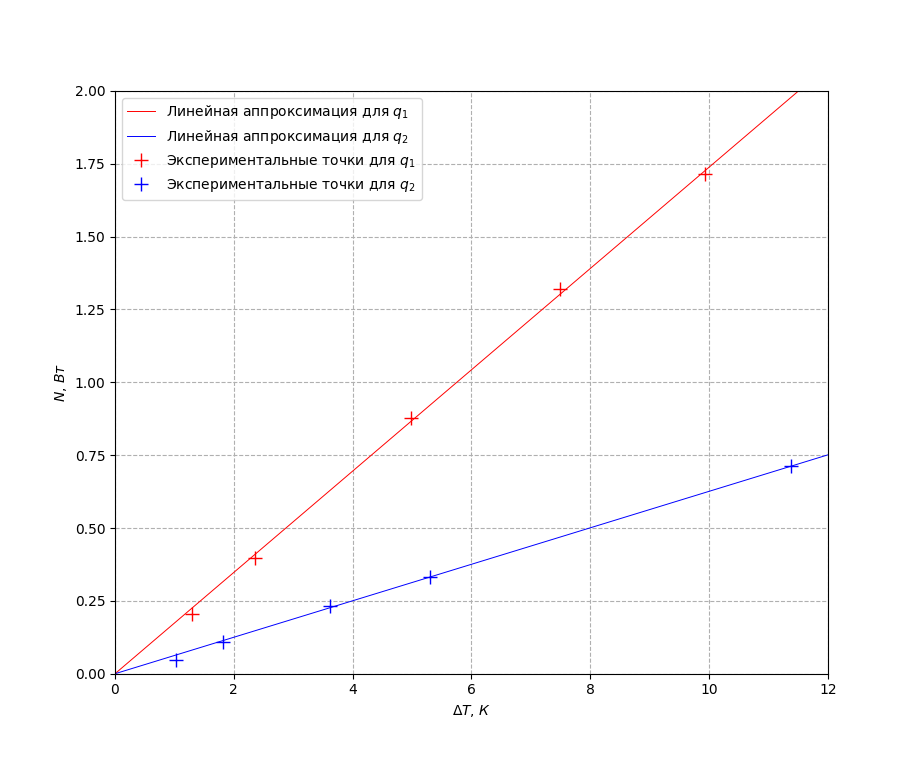
\includegraphics[width=1.1\textwidth]{graph.png}
	\caption{\textit{График зависимости $N$ от $\Delta T$ для обоих наборов измерений}}
	\label{graph}
\end{figure}


\subsection{Вычисление молярной теплоёмкости и мощности теплопотерь}

Теперь, имея соотношение вида $N = k \Delta T$, из соотношения \eqref{find-a} получаем

\begin{equation}
    k_i = C_p q_i + \alpha, \ \ \ i = 1, 2
\end{equation}

Отсюда находим значение $C_p$:

\begin{equation}
    C_p^\text{г} = \frac{k_2 - k_1}{q_2 - q_1} = \frac{0,063 - 0,174}{0,0475 - 0,172} = 0,90 \ \frac{\text{Дж}}{\text{К} \cdot \text{г}}
\end{equation}

Погрешность вычисления $C_p$ можно вычислить по формуле:

\begin{multline*}
    \sigma_{C_p^\text{г}} = \sqrt{
    \left( \frac{\partial C_p}{\partial k_1} \right)^2 \sigma_{k_1}^2 + 
    \left( \frac{\partial C_p}{\partial k_2} \right)^2 \sigma_{k_2}^2 + 
    \left( \frac{\partial C_p}{\partial q_1} \right)^2 \sigma_{q_1}^2 + 
    \left( \frac{\partial C_p}{\partial q_2} \right)^2 \sigma_{q_2}^2
    } = \\
    = \sqrt{
    \left( \frac{\sigma_{k_1}}{q_2 - q_1} \right)^2 + \left( \frac{\sigma_{k_2}}{q_2 - q_1} \right)^2 + 
    \left( \frac{\sigma_{q_1} (k_1 - k_2)}{(q_1 - q_2)^2} \right)^2 + 
    \left( \frac{\sigma_{q_2} (k_1 - k_2)}{(q_1 - q_2)^2} \right)^2
    } = \\
    = \frac{1}{q_1 - q_2} \sqrt{
    \sigma_{k_1}^2 + \sigma_{k_2}^2 + \left( \frac{k_1 - k_2}{q_1 - q_2} \right)^2 \left( \sigma_{q_1}^2 + \sigma_{q_2}^2 \right)
    } = \frac{1}{q_1 - q_2} \sqrt{
    \sigma_{k_1}^2 + \sigma_{k_2}^2 + C_p^2 \left( \sigma_{q_1}^2 + \sigma_{q_2}^2 \right)
    }
\end{multline*}

\begin{equation}
    \sigma_{C_p^\text{г}} = \frac{1}{0,172 - 0,0475} \sqrt{
    0,001^2 + 0,001^2 + 0,9^2 \left( 0,001^2 + 0,0001^2 \right)
    } \approx 0,01 \ \frac{\text{Дж}}{\text{К} \cdot \text{г}}
\end{equation}

Таким образом $C_p^\text{г} = (0,90 \pm 0,01) \ \text{Дж}/(\text{К} \cdot \text{г})$ (в рассчёте на один грамм). Молярная теплоёмкость тогда

\begin{equation}
    C_p = C_p^\text{г} \cdot \mu = (0,90 \pm 0,01) \cdot 29,0 = (26,0 \pm 0,4) \ \frac{\text{Дж}}{\text{К} \cdot \text{моль}}
\end{equation}

Теперь можно посчитать значение коэффициента $\alpha = k_i - C_p q_i$, $i$ = 1, 2. Очевидно, что $\alpha_1 = \alpha_2$, тогда положим 

\begin{equation}
    \alpha = \alpha_1 = k_1 - C_p^\text{г} q_1 = 0,174 - 0,90 \cdot 0,172 = 0,020 \ \frac{\text{Вт}}{\text{К}}
\end{equation}

Погрешность вычисления $\alpha$ можно рассчитать по формуле

\begin{multline*}
    \sigma_\alpha = \sqrt{\sigma_{k_1}^2 + \left( \frac{\partial \alpha}{\partial C_p} \right)^2 \sigma_{C_p}^2 + 
    \left( \frac{\partial \alpha}{\partial q_1} \right)^2 \sigma_{q_1}^2
    } = \sqrt{
    \sigma_{k_1}^2 + q_1^2 \sigma_{C_p}^2 + C_p^2 \sigma_{q_1}^2
    } = \ \ \ \ \ \ \ \ \ \ \ \ \ \ \ \ \ \ \ \ \ \ \ \ \ \ \ \ 
\end{multline*}

\begin{equation}
    = \sqrt{0,001^2 + 0,172^2 \cdot 0,01^2 + 0,9^2 \cdot 0,001^2 } = 0,003 \ \frac{\text{Вт}}{\text{К}}
\end{equation}

Таким образом

\begin{equation}
    \alpha = (0,020 \pm 0,003) \ \frac{\text{Вт}}{\text{К}}
\end{equation}

Из соотношений \eqref{loss} и \eqref{find-a} следует, что

\begin{equation}
    \frac{N_\text{пот}}{N} = \frac{\alpha}{k}
\end{equation}

Тогда посчитает это отношение для двух значений расходов газа и запишем в таблицу \ref{q-loss}.

\begin{table}[!ht]
    \centering
    \begin{tabular}{|l|l|l|}
    \hline
        $q$, г/с & $\frac{N_\text{пот}}{N}$ & $\sigma_x$ \\ \hline
        0,172 & 0,12 & 0,01 \\ \hline
        0,0475 & 0,32 & 0,04 \\ \hline
    \end{tabular}\caption{\textit{Вычисление доли потерь для обоих значений расхода}}\label{q-loss}
\end{table}

Погрешность вычисления отношения можно посчитать по формуле (пусть $x = N_\text{пот}/N$)

\begin{equation}
    \sigma_x = \sqrt{
    \left( \frac{\partial x}{\partial \alpha} \right)^2 \sigma_{k_1}^2 + 
    \left( \frac{\partial x}{\partial k} \right)^2 \sigma_{k_1}^2 
    } = \sqrt{
    \frac{\sigma_\alpha^2}{k^2} + \frac{\alpha^2 \sigma_k^2}{k^4}
    } = \frac{1}{k} \sqrt{
    \sigma_\alpha^2 + \frac{\alpha^2 \sigma_k^2}{k^2}
    } = \frac{1}{k} \sqrt{\sigma_\alpha^2 + x^2 \sigma_k^2}
\end{equation}

Теперь вычислим погрешность для обоих значений $x$ и запишем в таблицу \ref{q-loss}.

\section{Обсуждение результатов и выводы}

В ходе работы была измерена удельная теплоёмкость воздуха при постоянном давлении $C_p = (26,0 \pm 0,4) \ \text{Дж}/\text{моль} \cdot \text{г}$. Теоретическое значение $C_p^\text{теор} = 29,09 \ \text{Дж}/\text{К} \cdot \text{моль}$. Табличное значение при данной температуре воздуха составляет $C_p^\text{табл} = 29,15 \ \text{Дж}/\text{К} \cdot \text{моль}$. Видно, что разница экспериментального значения с табличным и теоретическим превышает погрешность вычисления, значит эксперимент был проведён не очень точно или используемая модель газа не соответствует действительности.

Расхождение результата можно объяснить несколькими способами:

\begin{enumerate}
    \item Из-за того, что время в лаборатории ограничено, а для установления теплового равновесия требуется много времени, полученные значения приборов не вполне подходят для измерений
    \item Воздух не является смесью двухатомных идеальных газов, так как в нём присутствуют другие газы, а также водяной пар (влажность воздуха во время опытов была $\varphi = 23,2 \%$)
\end{enumerate}

\end{document}